\section{ODD for StationSim GCS}
\label{sec:stationsim}

\subsection{Overview}
\label{sub:stationsim:overview}

\subsubsection{Purpose and patterns}
\label{subs:stationsim:overview:purpose}

StationSim GCS is an updated version of the StationSim model.
The original StationSim aimed to simulate the motion of pedestrians across a
hypothetical rectangular station with 3 entrances on one side and 2 exits on the
opposite side as shown in Figure \ref{fig:stationsim_env}.
The new StationSim GCS also aims to simulation the motion of pedestrians across
a station; however, in this case the model is based on the real-world example of
Grand Central Station in New York, focusing specifically on the concourse area
highlighted in Figure \ref{fig:gcs_concourse}.
This is reflected in the simulation environment shown in Figure
\ref{fig:stationsim_gcs_env}.
The environment consists of X gates which act simultaneously as both entrances
and exits.
Each pedestrian in the simulation is assigned an entrance and an exit and, upon
entering the environment, seeks to move as directly as possible towards their
assigned exit without colliding with other pedestrians.
Where collisions are more likely to occur (e.g. close to entrances/exits and
around solid obstacles), we typically observe crowding as population densities
increase.

\todo{What are the patterns}

\begin{figure}[h]
    \centering
    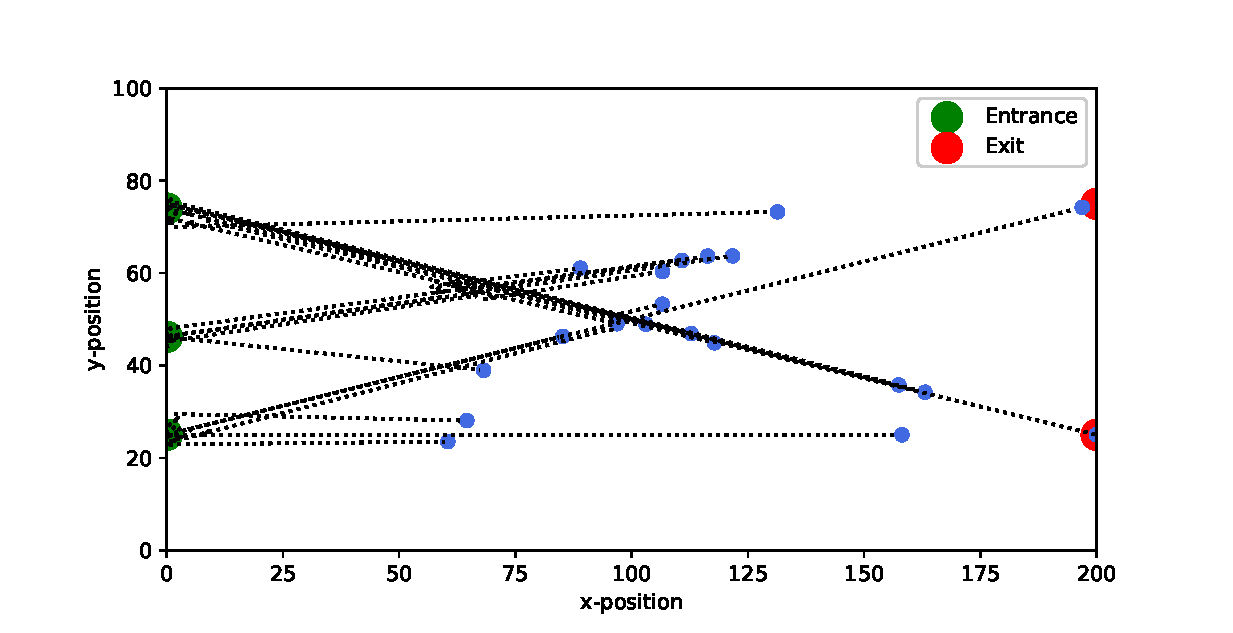
\includegraphics[width=0.7\textwidth]{sample_model_run}
    \caption{Layout of environment in original StationSim model.}

    \label{fig:stationsim_env}
\end{figure}

\begin{figure}[h]
    \centering
    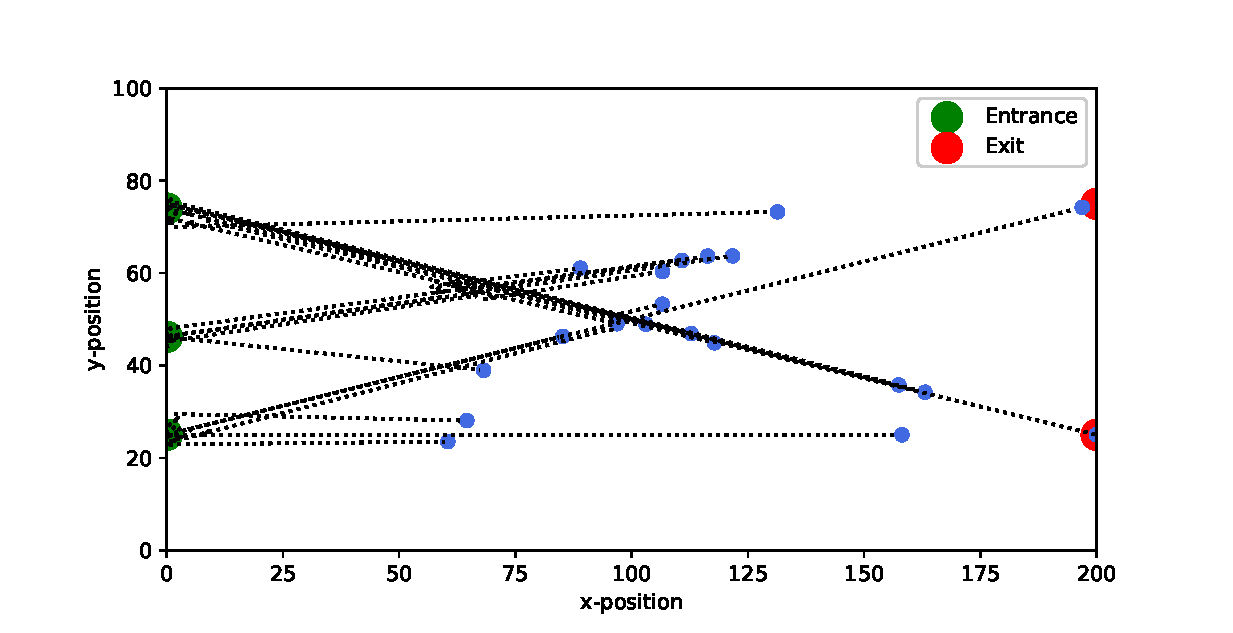
\includegraphics[width=0.7\textwidth]{sample_model_run}
    \caption{Layout of Grand Central Station concourse.}
    \label{fig:gcs_concourse}
\end{figure}

\begin{figure}[h]
    \centering
    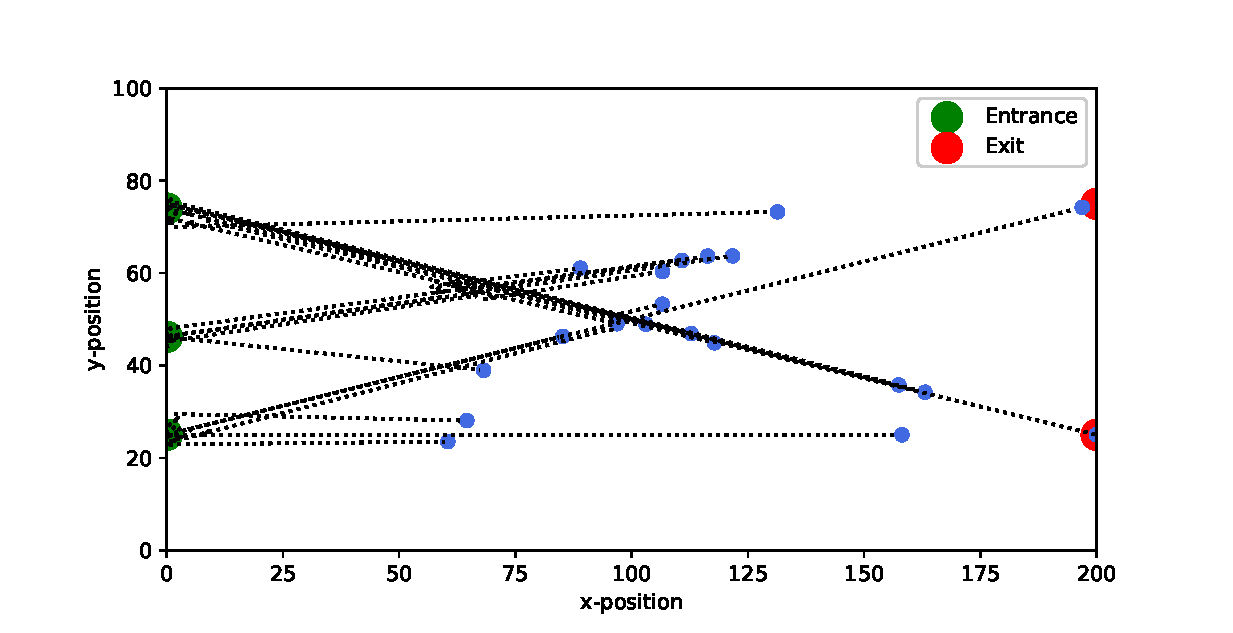
\includegraphics[width=0.7\textwidth]{sample_model_run}
    \caption{Layout of environment in StationSim GCS model.}
    \label{fig:stationsim_gcs_env}
\end{figure}

\subsubsection{Entities, state variables and scales}
\label{subs:stationsim:overview:entities}

The StationSim GCS model is made up of 4 different types of entities:
\begin{enumerate}
    \item Agents,
    \item The environment,
    \item Gates around the edge of the environment, and
    \item Obstacles in the environment.
\end{enumerate}
These entities aim to simulate the scenario outlined in Section
\ref{sub:stationsim:overview}.
The agents in this model represent pedestrians; these are portrayed as
two-dimensional circular entities with finite radius.
The variables pertaining to these agents can be found in Table
\ref{tab:agent_variables}.
The environment in this model represents the concourse of Grand Central Station
in New York; this is portrayed as two-dimensional continuous space bounded by
rectangular walls within which agents may move.
The model is designed such that the left-hand side of the environment
represents the South side of the concourse, the right-hand side the North side,
the top side the West side and the bottom side the East side.
The variables pertaining to the environment entity can be found in Table
\ref{tab:environment_variables}.

\begin{table}
    \centering
    \begin{tabularx}{\textwidth}{lX}
        \toprule
        Variable Name & Description \\
        \midrule
        \texttt{location} & Agent's $x$-$y$ coordinates in 2-dimensional
                            continuous space; bounded by the height and width of
                            the environment \\
        \texttt{status} & Agent's status; 0 indicates agent has not started, 1
                          indicates agent is active, 2 indicates agent has
                          finished \\
        \texttt{size} & Radius of agent's circular body \\
        \texttt{speed} & Agent's speed; indicative of the distance covered by an
                         agent in a single time-step \\
        \texttt{unique\_id} & Unique numerical identifier for a specific agent
                              in a model \\
        \texttt{gate\_in} & Number of the gate through which of the gates the
                            agent enters the environment ($0 \leq n \leq 9$) \\
        \texttt{gate\_out} & Number of the gate through which of the gates the
                             agent exits the environment ($0 \leq n \leq 9$) \\
        \texttt{loc\_desire} & $x$-$y$ coordinate of the agent's target
                               destination; defined by taking the $x$-$y$
                               coordinates of \texttt{gate\_out} and adding some
                               uniformly distributed random noise \\
        \bottomrule
    \end{tabularx}
    \caption{Table of state variables pertaining to gate entities.}
    \label{tab:agent_variables}
\end{table}

\begin{table}
    \centering
    \begin{tabularx}{\textwidth}{lX}
        \toprule
        Variable Name & Description \\
        \midrule
        \texttt{height} & Environment's height \\
        \texttt{width} & Environment's width \\
        \texttt{gates\_in} & Number of gates through which agents can enter the
                             environment \\
        \texttt{gates\_out} & Number of gates through which agents can exit the
                              environment \\
        \bottomrule
    \end{tabularx}
    \caption{Table of state variables pertaining to the environment entity.}
    \label{tab:environment_variables}
\end{table}

Along the edge of these boundaries are located gates: one gate is located on the
South side, five gates are located on the North side, two gates are located on
the West side and two gates are located on the East side.
The gates are points along the boundary of the environment at which agents may
either enter or exit.
These have specific fixed $x-y$ coordinates.
Upon initialisation, each agent is provided with a start gate and end gate, from
which it draws its initial location and target destination; in defining its
target destination, the agent introduces some random noise to the $x-y$
coordinate in order to emulate the non-zero width of the gate.
The variables pertaining to the gate entities can be found in Table
\ref{tab:gate_variables}.

\begin{table}
    \centering
    \begin{tabularx}{\textwidth}{lX}
        \toprule
        Variable Name & Description \\
        \midrule
        x & Agent's x-coordinate \\
        y & Agent's y-coordinate \\
        \bottomrule
    \end{tabularx}
    \caption{Table of state variables pertaining to agent entities.}
    \label{tab:gate_variables}
\end{table}

The environment also contains a single obstacle which represents a clock.
As shown in Figure \ref{fig:gcs_concourse}, this lies in the centre of the
concourse.
From a model architecture perspective, this obstacle is treated as a stationary
agent; other agents therefore treat it as they would any other agent and make
efforts to avoid colliding with it.
The variables pertaining to the obstacle entity can be found in Table
\ref{tab:obstacle_variables}.

\begin{table}
    \centering
    \begin{tabularx}{\textwidth}{lX}
        \toprule
        Variable Name & Description \\
        \midrule
        x & Agent's x-coordinate \\
        y & Agent's y-coordinate \\
        \bottomrule
    \end{tabularx}
    \caption{Table of state variables pertaining to the obstacle entity.}
    \label{tab:obstacle_variables}
\end{table}

\subsubsection{Process overview and scheduling}
\label{subs:stationsim:overview:process}

\todo{INSERT FLOW DIAGRAM OF OVERARCHING PROCESS OF MODEL}

\subsection{Design Concepts}
\label{sub:stationsim:design_concepts}

\todo{Which of these design concepts are involved in StationSim?}
\todo{Give a very brief of how each concept is relevant.}

\begin{enumerate}
    \item Basic principles
    \item Emergence
    \item Adaptation
    \item Objectives
    \item Learning
    \item Prediction
    \item Sensing
    \item Interaction
    \item Stochasticity
    \item Collectives
    \item Observation
\end{enumerate}

\subsection{Details}
\label{sub:stationsim:details}

\subsubsection{Initialisation}
\label{subs:stationsim:details:initialisation}

\subsubsection{Input data}
\label{subs:stationsim:details:input}

\subsubsection{Submodels}
\label{subs:stationsim:details:submodels}

